\documentclass[../book.tex]{subfiles}
\graphicspath{{\subfix{../images/}}}

\begin{document}
\chapter{Function Basics}
\begin{introduction}[Contents]
\item Basic Set Theory
\item Introduction to Functions
\item Inverse Functions
\item Transformations, End Behavior, and Graphing
\item Piece-wise Functions and Function Combinations
\end{introduction}
Functions are the basis of Algebra.  They take in some number of independent variables and output a dependent variable.  For the sake of this course, we will be mostly dealing with uni-variate functions; that is, functions with one input and one output.  Suppose you have a calculator that can only do one programmed set of operations.  For any number you put in, it triples it and adds one.  For example, inputting $3$ outputs $10$, inputting $5$ outputs $16$, etc.  We can define a function $f(x)=3x+1$ to represent the situation.  $f$ is the name of the function.  "$(x)$" means that the function is in terms of the independent \textit{dummy variable}, $x$.

There's not that much else to functions; they are super simple.  We define the function, input the value needed, and record the output.  Most functions are either written as $f(x)$ or $y(x)$.  If more than one function is being discussed at any one time, it is common to continue down the alphabet with $g(x)$, $h(x)$, etc.

In this chapter, we will go over the types of sets that exist in Algebra, then discuss the types of common functions, go over domain and range, discuss the inverse of a function and its application, and finally the meaning of a function transformation.
\section{Basic Set Theory}
\noindent Set Theory is, like it sounds, the application of mathematical logic to sets.  A \textit{set} is a collection of numbers, objects, or other sets.  In mathematics, it's most valuable to limit our sets to only contain numbers, but it can contain anything.  For example, the set of U.S.  states starting with the letter "A" is $$\{\text{Alabama, Alaska, Arizona, Arkansas}\}.$$
Here is an example of a numerical set: $$\{1,2,3,4,5,6,7,8,9,10,11,12\}.$$
\subsection{Definitions}
This section will cover the definitions needed for this chapter.  There are a lot.  Please read through them because they will be referred to throughout the book.  

Here is a list of the most common sets in mathematics.  These will be referred to often throughout the book, so it is important that you know the definition of the set and its notation.

The \textit{real set} is the set of all real numbers.  A \textit{real number} is any number that doesn't have an imaginary component.  Complex numbers will be detailed in \hyperlink{chapter.3}{Chapter 3}.  The real set is denoted as $\mathbb{R}$.  An example of a set of real numbers (not the real set!) is $\displaystyle \left\{1,\sqrt{2},\frac{11}{3},-12,\pi\right\}$.

The \textit{integer set} is the set of all integers.  An \textit{integer} is any number that doesn't have a fractional component.  These can be positive,negative, or zero.  The integer set is denoted as $\mathbb{Z}$.  An example set of integers is $\{-2,4,-78,12\}$.

The \textit{rational set} is the set of all rational numbers.  A \textit{rational number} is any number that can be represented as a fraction with an integer numerator and denominator.  Because of this restriction, $e$, $\pi$, and the square root of any non-perfect square (such as $2,3,5,6,7,\ldots$) is an \textit{irrational number} because they cannot be expressed as a ratio of two integers.  The rational set is denoted as $\mathbb{Q}$.  An example set of rational numbers is $\displaystyle \left\{-1,4.7,\frac{11}{2},\sqrt{36}\right\}$.

The \textit{natural set} is the set of all natural numbers.  A \textit{natural number} is a counting number - it's any positive integer.  Remember that zero does not count as positive! The notation for the natural set is $\mathbb{N}$.  An example set of natural numbers is $\{2,5,13,69\}$.

The \textit{complex set} is the set of all complex numbers.  A \textit{complex number} is any number that can be written as $a+bi$, for real numbers $a$ and $b$, and $i$ as the imaginary constant.  We won't worry about complex numbers until \hyperlink{chapter.3}{Chapter 3}, but it's good to put them in the list.  The notation for the complex set is $\mathbb{C}$.

Here are some more definitions that will be used throughout the book.  These refer to the properties of a set:

An \textit{element} is a value of a set.  Whether this be a number, idea, object, or another set, it's one of the components of the set.  For example, $2$ is an element of the set $\{1,2,3,4,5\}$.  We have a notation to describe this: "$\in$".  So, we could say $2\in\{1,2,3,4,5\}$ (read as "$2$ is in the set $\{1,2,3,4,5\}$).

A \textit{subset} describes a set that whose elements are all in another set.  In order words, we say that set \textbf{A} is a subset of set \textbf{B} if every element of set \textbf{A} is an element of set \textbf{B}.  We use the notation $\subseteq$ for subsets.  For example, we can say that $\mathbb{N}\subseteq\mathbb{Z}$ since every member of the natural set is in the integer set.  A \textit{proper subset} is a subset such that \textbf{A}$\neq$\textbf{B}.  This means that every element of \textbf{A} is in \textbf{B} but \textbf{B} has elements that aren't in \textbf{A}.  As a result, $\mathbb{N}_0\subseteq\mathbb{W}$ - since the natural numbers plus zero becomes the whole number set - while $\mathbb{N}\subset\mathbb{R}$.

The \textit{null set}, sometimes referred to as the \textit{empty set}, is a set that contains no elements.  The notation for the empty set are $\varnothing$ or $\{\}$.

\begin{remark}
  Technically, the null set is a subset of every set.
\end{remark}

The final two definitions are the main operations that we can do to sets: union and intersection.  

The \textit{union} of two sets refers to the combination of every element in both sets.  It is represented by the symbol $\cup$ or the verbiage "or".  For example, if \textbf{A}$=\{1,4,7,10,13\}$ and \textbf{B}$=\{2,3,5,6,8,9,11,12\}$, then \textbf{A} $\cup$ \textbf{B} $=\{1,2,3,4,5,6,7,8,9,10,11,12,13\}$.

\begin{remark}
  If sets \textbf{A} and \textbf{B} have an element in common, it is only written once.
\end{remark}

The \textit{intersection} of two sets refers to the elements in common between two sets.  It is represented by the symbol $\cap$ or the verbiage "and".  For example, if \textbf{A}$=\{4,8, 12,16,20,24,28|\}$ and \textbf{B}$=\{5,10,15,20,25,30\}$, then \textbf{A}$\cap$\textbf{B}$=\{20\}$.
Let's look at an example to summarize this information:
\begin{example}
Given the following sets, find \textbf{A}$\cup$\textbf{B} and \textbf{A}$\cap$\textbf{B}.  Then determine if \textbf{A} is a subset of \textbf{B} (or vice versa) and prove whether \textbf{A} is a subset of the natural numbers.  \begin{align*}
    \text{\textbf{A}}&:=\text{The set of all multiples of 3 up to 30 (inclusive)} \\
    \text{\textbf{B}}&:=\text{The set of all even numbers up to 30 (inclusive)}
\end{align*}
\end{example}
\begin{solution}
Here is the lists described in the problem: \begin{align*}
    \text{\textbf{A}}&=\{3,6,9,12,15,18,21,24,27,30\} \\
    \text{\textbf{B}}&=\{2,4,6,8,10,12,14,16,18,20,22,24,26,28,30\}
\end{align*}
The first two parts are very easy and require little explanation: \begin{align*}
\text{\textbf{A}}\cup\text{\textbf{B}}&=\{2,3,4,6,8,9,10,12,14,15,17,18,20,21,22,24,26,27,28,30\} \\
\text{\textbf{A}}\cap\text{\textbf{B}}&=\{6,12,18,24,30\}
\end{align*}
The second two parts require more of an explanation.  Noting that \textbf{A} has elements that aren't in \textbf{B} (such as $2$), and \textbf{B} has elements that aren't in \textbf{A} (such as $3$), neither sets are a subset of the other.  Since every element of \textbf{A} is a natural number, and \textbf{A} is not the natural set, we can say that \textbf{A}$\subset\mathbb{N}$.$\Box$
\end{solution}
\noindent Those are all the definitions needed, so let's talk about interval notation.
\subsection{Interval Notation}
\noindent Interval notation is one of the most used answer formats in Algebra.  Teachers will often require it as it's easy to read and very descriptive.  Interval notation describes a range of data; it gives every interval where the data follows a certain condition (whether it be a given inequality or the solution to an equation, etc.) In interval notation, there are two important symbols that we use:  \begin{align*}
    (\text{ }) &:= \text{the number is not included in the set} \\
    [\text{ }] &:= \text{the number is included in the set}
\end{align*}
Let's take a look at a number of examples to get a better understanding of the notation.
\begin{example}
Write $x>7$ in interval notation.
\end{example}
\begin{solution}
To write in interval notation, we need the bounds of the inequality.  Clearly, the lower bound is $7$.  But what is the upper bound?  Well, it's $+\infty$!.  We also need to note whether we need to include the bounds.  We don't include $7$ because it's a $>$, not $\geq$.  Since $+\infty$ is technically not reachable, we never include that.  So, our interval notation, is $(7,\infty)$.$\Box$
\end{solution}
\noindent That last part is very important to remember.  Let's put it in a note.
\begin{note}
If a bound is $\pm\infty$, since it's impossible to reach, we \textit{always} put an open parenthesis.
\end{note}
\begin{example}
Write $7<x\leq 12$ in interval notation.
\end{example}
\begin{solution}
Our bounds are $7$ and $12$.  Since $7$ is not included, and $12$ is, we say that the interval notation is $(7,12]$.$\Box$
\end{solution}
\noindent Now, let's look at an example involving more than one interval.
\begin{example}
Write $x \leq 6$ or $7<x\leq 12$ in interval notation.  
\end{example}
\begin{solution}
We consider the intervals separately.  The first interval is $(-\infty,6]$ and the second is $(7,12]$.  All we need to do is put them together, since "or" was used, using the union notation, so our interval is $(-\infty,6]\cup(7,12]$.  $\Box$
\end{solution}
\begin{example}
Write $x\leq 12$ and $x=11$ in interval notation.
\end{example}
\begin{solution}
The intersection between these two intervals is $x=11$, so the interval is just $[11]$.$\Box$
\end{solution}
\begin{example}
Write $x\geq 12$ and $x=11$ in interval notation.
\end{example}
\begin{solution}
There is no intersection point, so we can write the answer as $\varnothing$.$\Box$
\end{solution}
\noindent With these two pieces out of the way, let's move on to discuss the most important topic in this chapter: functions.
\section{Introduction to Functions}
\noindent A \textit{function} takes in a value or an input and spits out a value or an \textit{output}.  The reason sets are important is that the input for continuous functions consists of a set of numbers, while the output is also a set of numbers that correspond to the input.

You'll often see a table as shown in the examples below.  The $x$ section represents the input or the $x$-value that is being plugged in.  $f$ represents the actual function functioning on $x$ and $f(x)$ represents the output value.
\begin{example}
Write a table to show the values of $f(x)=x+1$ at $x=0,1,2$.
\end{example}
\begin{solution}
In this case, this function says for every input, add $1$ to find the output.
\begin{center}
\begin{tabular}{ |c|c|c| } 
 \hline
 $x$ & $f(x)=x+1$ & $f(x)$ \\ 
 \hline
 $0$ & $(0)+1$ & $f(0)=1$ \\ 
 $1$ & $(1)+1$ & $f(1)=2$ \\
 $2$ & $(2)+1$ & $f(2)=3$ \\
 \hline
\end{tabular}
\end{center}$\Box$
\end{solution}
\begin{example}
Write a table to show the values of $f(x)=x^2+1$ at $x=0,1,2$.
\end{example}
\begin{solution}
\begin{center}
\begin{tabular}{ |c|c|c| } 
 \hline
 $x$ & $f(x)=x^2+1$ & $f(x)$ \\ 
 \hline
 $0$ & $(0)^2+1$ & $f(0)=0$ \\ 
 $1$ & $(1)^2+1$ & $f(1)=2$ \\
 $2$ & $(2)^2+1$ & $f(2)=5$ \\
 \hline
\end{tabular}
\end{center}$\Box$
\end{solution}
\noindent The definition of a function given above is an over-simplified definition of a function.  Let's take a look at the formal definition of a function.

A function is any function that has only one output for every input.  In other words, this function passes the \textit{vertical-line test}.  If you look at the examples above, every input has \textit{one} output.  

Here's an example of something that doesn't have one input.
\begin{example}
Write a table to show the values of $f(x)=\pm\sqrt{x}$ at $x=0,1,2$.
\end{example}
\begin{solution}
\begin{center}
\begin{tabular}{ |c|c|c| } 
 \hline
 $x$ & $f(x)=\pm\sqrt{x}$ & $f(x)$ \\ 
 \hline
 $0$ & $\pm\sqrt{(0)}$ & $f(0)=0$ \\ 
 $1$ & $\pm\sqrt{(1)}$ & $f(1)=-2$ and $f(1)=1$ \\
 $2$ & $\pm\sqrt{(2)}$ & $f(2)=-\sqrt{2}$ and $f(2)=\sqrt{2}$ \\
 \hline
\end{tabular}
\end{center}$\Box$
\end{solution}
\begin{wrapfigure}{r}{4cm}
    \begin{tikzpicture}[xscale=0.5,yscale=0.5]
      \draw[<->] (-3,0) -- (3,0) node[right] {$x$};
      \draw[<->] (0,-3) -- (0,3) node[above] {$y(x)$};
      \draw[scale=0.5,domain=-2.75:2.75,smooth,variable=\y,blue] plot ({\y*\y},{\y});
      \draw[dashdotted] (2,-3) -- (2,3);
    \end{tikzpicture}
\end{wrapfigure}
If we graphed the above function, it would look like the graph to the right.

As we can see, if we were to plug in any number (except $x=0$), it would yield two outputs.  Thus, this isn't a function as it doesn't pass the test.  

To see the vertical line test in action, simply draw a vertical line through a given function.  If it passes through more than one point, it isn't a function.  On the graph to the right, the dashed line represents an example of a vertical line that proves it to not be a function.  Only one example is necessary to prove this (though there are infinite cases in this example).

Before we continue, we need to establish two more terms: \textit{domain} and \textit{range}.  The input column is formally known as the domain and the output columns is the range.  These are described with the same interval notation as seen in the \hyperlink{section.2.1}{previous} section.
\begin{note}
The domain consists of all inputs, or $x$-values, that can be plugged into the function.  The range consists of all outputs, or $y$-values, that can be received from the function.
\end{note}
Note the use of the word "can".  This means that there are circumstances in which you cannot plug in $x$, meaning there is no corresponding $y$.

Here are some examples to further understand domain and range.
\begin{example}
Determine the domain and range of the function $f(x)=x^2$.
\end{example}
\begin{solution}
The domain asks what can be plugged into the function.  Is there anything that can't?  Nope!  So the domain can be written as $x\in\mathbb{R}$ or $x\in(-\infty,\infty)$.

Now, what can we receive from the function?  We can plug in some numbers and look for a generalization.  $0 \to 0$, $1 \to 1$, $-1 \to 1$, $\ldots$.  We see that the outputs can never be negative (try and prove it for yourself!).  This means that the range is $y\in[0,\infty)$.$\Box$
\end{solution}
\begin{example}
Determine the domain and range of the function $f(x)=\sqrt{x}$.
\end{example}
\begin{solution}
Since we can't take the square root of a negative number, the domain must be $x\in[0,\infty]$.

Experimenting with some values, we see that the return value can never be negative.  Thus, the range is $y\in[0,\infty)$.$\Box$
\end{solution}
\begin{example}
Determine the domain range of the function $f(x)=\dfrac{1}{x}$.
\end{example}
\begin{solution}
Because we can't divide by zero, the domain is $x\in(-\infty,0)\cup(0,\infty)$.

Since the function never reaches zero (plug in small values around zero like $0.1$, $0.001$, $-0.01$, etc.), the range is $y\in(-\infty,0)\cup(0,\infty)$.$\Box$
\end{solution}
Now that we've discussed the vertical line test, you must be wondering: is there a horizontal line test?  To answer that question, why yes there is! So, what is the purpose of the horizontal line test? The horizontal line test tests if a function is \textit{one-to-one}.  In other words, for every output, there is only one corresponding input.  
\begin{definition}{One-to-One Functions}{onetoone}
A \textit{one-to-one function} is a function where it and its inverse are functions.  This means that there is one input for every output and one output for every input (hence the name one-to-one).
\end{definition}
\begin{wrapfigure}{r}{4cm}
    \begin{tikzpicture}[xscale=0.5,yscale=0.5]
      \draw[<->] (-3,0) -- (3,0) node[right] {$x$};
      \draw[<->] (0,-3) -- (0,3) node[above] {$y(x)$};
      \draw[scale=0.5,domain=-2.75:2.75,smooth,variable=\x,blue] plot ({\x},{\x*\x});
      \draw[dashdotted] (-3,2) -- (3,2);
    \end{tikzpicture}
\end{wrapfigure}
We will discuss inverse functions in the \hyperlink{section.2.3}{next} section.

Lets look at two examples of the horizontal line test.
\begin{example}
Conduct the horizontal line test on $f(x)=x^2$ and analyze the results.
\end{example}
\begin{solution}
We are looking for at least one example where a horizontal line touches more than one point.  We see that there are an infinite points ($y=2$ is shown to the right), so this is not a one-to-one function.  There are two inputs for the same output.  $\Box$
\end{solution}
\begin{example}
Conduct the horizontal line test on $f(x)=x$ and analyze the results.
\end{example}
\begin{remark}
  Note that if an equation passes the horizontal line test, that doesn't always mean that it's one-to-one.  It \textbf{must} pass BOTH the horizontal and vertical line tests to be considered a function.
\end{remark}
\begin{solution}
We look for a horizontal line that touches more than one point and cannot find one.  This means that that $f(x)$ is a one-to-one function.  An example line at $y=2$ is plotted; every example line would look the exact same.  (The graph is shown on the next page.)$\Box$
\end{solution}
\newpage
\begin{wrapfigure}{r}{4cm}
    \begin{tikzpicture}[xscale=0.5,yscale=0.5]
      \draw[<->] (-3,0) -- (3,0) node[right] {$x$};
      \draw[<->] (0,-3) -- (0,3) node[above] {$y(x)$};
      \draw[scale=0.5,domain=-5:5,smooth,variable=\x,blue] plot ({\x},{\x});
      \draw[dashdotted] (-3,2) -- (3,2);
    \end{tikzpicture}
\end{wrapfigure}
Why is this important?  We are going to look at the importance in the next section when we discuss inverse functions.
\section{Inverse Functions}
\noindent Inverse functions were informally (and superficially) covered in Algebra I via a basic process.  Our goal in this section is to define an inverse function, how to find an inverse function, and understand the visual depiction of an inverse function and its relation to the starting function.

An inverse function is formally defined as $$f^{-1}\left(f(x)\right)=f\left(f^{-1}(x)\right)=x.$$
What this means is that the functions $f$ and $f^{-1}$ (the inverse of $f(x)$) are inverses if they satisfy the statement above.  But how do we find that?  Also, what does this mean graphically?

Let's discuss the first question.  Here is a guide to finding the inverse of a given function $f(x)$: \begin{enumerate}
    \item Replace $f(x)$ with $y$.
    \item Switch every $x$ with $y$ and vice-versa.
    \item Solve this equation for $y$ in terms of $x$.
    \item Replace this $y$ with $f^{-1}(x)$.
\end{enumerate}
Let's look at a few examples to better understand the process.
\begin{example}
Find $f^{-1}(x)$ if $f(x)=2x-3$.
\end{example}
\begin{solution}
We are going to follow the steps rigorously.
\begin{center}
    \begin{tabular}{c c}
        Step 1 & $y=2x-3$ \\
        Step 2 & $x=2y-3$ \\
        Step 3 & $\dfrac{x+3}{2}=y$ \\
        Step 4 & $f^{-1}(x)=\dfrac{x+3}{2}$
    \end{tabular}
\end{center}
We can check this: $\displaystyle 2\left(\dfrac{x+3}{2}\right)-3=x+3-3=x$.  This means we have it right.  $\Box$
\end{solution}
\begin{example}
If $f(x)=x^2$, find $f^{-1}(x)$.
\end{example}
\begin{solution}
Switching $x$ and $y$ we get $x=y^2$, which means that $f^{-1}(x)=\pm\sqrt{x}$.  $\Box$
\end{solution}
\begin{note}
It is really important that you do \textbf{not} forget the "$\pm$"!  When we do square roots, always write it and then determine if it's necessary.  That holds true for the rest of your career in mathematics.
\end{note}
This example brings up an important point.  We proved in the \hyperlink{section.2.2}{previous} section that the inverse function isn't a function!  How is this possible?  How can the inverse of a function not be a function?  To explain this, we must define the graphical definition of an inverse function.

Using example 2.15, lets make a table of inputs and outputs for the function and its inverse.
\begin{table}[!htbp]
\centering
\begin{tabular}{|c|c|c|c|}
\hline
\multicolumn{2}{c}{$f(x)=2x-3$} & \multicolumn{2}{c}{$f^{-1}(x)=\dfrac{x+3}{2}$}\\
\hline
Input   & Output   & Input    & Output   \\
$-1$ & $-5$ & $-1$ & $1$  \\
$0$  & $-3$ & $0$  & $3/2$  \\
$1$  & $-1$ & $1$  & $2$  \\
$2$  & $1$  & $2$  & $5/2$ \\
$3$  & $3$  & $3$  & $3$ \\
$4$  & $5$  & $4$  & $7/2$ \\
\hline
\end{tabular}
\end{table}
\begin{wrapfigure}{r}{4cm}
    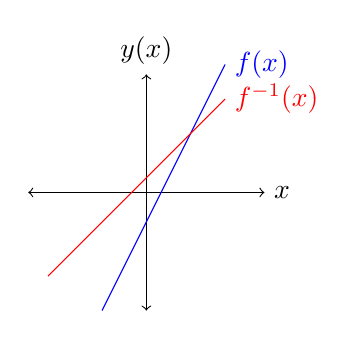
\begin{tikzpicture}[xscale=0.25,yscale=0.25]
      \draw[<->] (-6,0) -- (6,0) node[right] {$x$};
      \draw[<->] (0,-6) -- (0,6) node[above] {$y(x)$};
      \draw[scale=0.5,domain=-4.5:8,smooth,variable=\x,blue] plot ({\x},{2*\x-3}) node[right] {$f(x)$};
      \draw[scale=0.5,domain=-10:8,smooth,variable=\x,red] plot ({\x},{\x+3/2}) node[right] {$f^{-1}(x)$};
    \end{tikzpicture}
\end{wrapfigure}
If you look closely at the inputs and outputs of the original function and its inverse, you might notice something.  The inputs and outputs are switched!  This means that whenever you take the inverse, you are quite literally flipping the $x$-values and $y$-values in a table.  Graphically, here's what this looks like.

We see that the graphs intersect.  This is okay!  Sometimes they do, other times they don't.  Below we put two more examples of functions and their inverse.
\begin{figure}[!h]
    \centering
    \begin{tikzpicture}[xscale=0.35,yscale=0.35]
      \draw[<->] (-6,0) -- (6,0) node[right] {$x$};
      \draw[<->] (0,-6) -- (0,6) node[above] {$y(x)$};
      \draw[scale=1,domain=-6:1.25,smooth,variable=\x,blue] plot ({\x},{exp(\x)}) node[right] {$f(x)$};
      \draw[scale=1,domain=0.01:6,smooth,variable=\x,red] plot ({\x},{ln(\x)}) node[right] {$f^{-1}(x)$};
    \end{tikzpicture}   
    \begin{tikzpicture}[xscale=0.35,yscale=0.35]
      \draw[<->] (-6,0) -- (6,0) node[right] {$x$};
      \draw[<->] (0,-6) -- (0,6) node[above] {$y(x)$};
      \draw[scale=1,domain=-1.8:1.8,smooth,variable=\x,blue] plot ({\x},{\x*\x*\x}) node[right] {$f(x)$};
      \draw[scale=1,domain=-1.8:1.8,smooth,variable=\y,red] plot ({\y*\y*\y},{\y}) node[right] {$f^{-1}(x)$};
    \end{tikzpicture}   
\end{figure}
The first graph is of the exponential and logarithmic functions.  These will be reviewed in \hyperlink{chapter.9}{Chapter 9}.  The second graph is of the cubic and cube root functions.  These will be covered in \hyperlink{section.6.2}{Section 6.2} and \hyperlink{section.8.4}{Section 8.4}.

These graphs seem to display some sort of symmetry.  It seems that they are all reflected about a line.  Which line? It's $y(x)=x$.  So, if you reflect a function about the line $y(x)=x$, you obtain a function's inverse.  But why?

Remember that we switched the $x$-values and $y$-values when calculating the inverse.  This means that $x=y$, which means that it must relate to the line $y(x)=x$.

Now let's address the question of why we do this.  In the formal definition of the inverse, if you plug the inverse into the original function or vice versa, we obtain $x$.  Looking at the equation $f\left(f^{-1}(x)\right)=x$ and take the inverse of both sides, we obtain $f^{-1}(x)=f^{-1}(x)$.  This means that the formal definition of an inverse confirms the fact that these functions are equal.  The function reflects itself if the statement holds true, and as a result, when you reflect about the line $y(x)=x$, you obtain the inverse.

Another reason is the concept of reflection.  Whenever you reflect something about a point or line the overall distance from that point or line remains constant.  Thus, in order to obtain the point that is equidistant to the line $y(x)=x$, or an equation that is equidistant to the line $y(x)=x$, you have found that original equation’s inverse.  

The final reason involves the graphs.  It’s as if you combined the equations or plugged them into one another, their curves and anything deviating from the line would cancel and only leave the line of reflection $y(x)=x$, which is exactly what happens in the formal definition.  Only the inverse function can accomplish this.

Why was the horizontal line test important in determining the existence of an inverse?  It seems like we left this out.

Well, if you look at the second example for finding an inverse you’ll see why.  The function $f(x) = x^2$ isn't one-to-one and doesn't pass the horizontal line test.  This means there is more than one input for one output.  Well, when you take the inverse, it switches the inputs and outputs.  So that means there is more than one output for one input in the inverse function.  But wait! We can’t have more than one output for one input, because that means it isn't a function! And this is why the horizontal-line test is important.  It confirms the existence of not only an inverse, but an \textit{inverse function}.

Another way to think about is the concept of reflecting across the line $y(x)=x$.  The horizontal line test for a function is the vertical line test for an inverse function and vice-versa.  

One last question: What about the domain and range of an inverse function?  Well, if the input and outputs switch from original to inverse, that means the domain and range’s switch as well!
\begin{example}
Find the domain and range of $f(x)=\sqrt{x}$ and its inverse.
\end{example}
\begin{solution}
In the \hyperlink{section.2.2}{previous} section we found the domain and range of $f(x)$ to be $x\in[0,\infty)$ and $y\in[0,\infty)$.  If we find the inverse of $f(x)$, we get $y=\sqrt{x} \implies x=\sqrt{y}\implies f^{-1}(x)=x^2$.  The domain and range of this is $x\in[0,\infty)$ and $y\in[0,\infty)$.  $\Box$
\end{solution}
Now this example brings up an interesting point about obtaining inverse functions.  In an earlier example in this section, we said the inverse of $f(x)=x^2$ isn't a function because $x^2$ didn't pass the horizontal line-test.  So why does $f(x) = \sqrt{x}$ have an inverse that is equal to $x^2$ but, $x^2$ doesn't have an inverse? The trick here comes down to the domain.  If we notice, the domain of  $\sqrt{x}$ range only extends from $0$ to infinity.  Thus, the domain of the resulting inverse extends from $0$ to infinity as well.  Thus, in order to make the inverse of $x^2$ a legitimate function, we have to \textit{restrict its domain}.
\begin{note}
If you restrict a function’s domain such that it is one-to-one on that domain, it has an inverse function on that domain.  
\end{note}
With this, we conclude our introduction to inverse functions.  Throughout the book, we will learn about even more functions, some which may be invertible, and some which have even more going on than what is in this section.  Now, let' talk about function transformations.
\section{Transformations, End Behavior, and Graphing}
\noindent In this section, we will go into all the possible things that can affect the end-behavior of a function.  Like the set-notation section, this section may be very definition heavy.

The $y$-intercept is where the function crosses the $y$-axis.  To obtain it, let $x=0$ and solve for $y$.  The $x$-intercept is where the function crosses the $x$-axis.  To obtain it, let $y=0$ and solve for $x$.

Let's look at an example of this.
\begin{example}
Find the $x$- and $y$-intercepts of $f(x)=x^2$.
\end{example}
\begin{solution}
Letting $x=0$, we get the $y$-intercept as $f(0)=(0)^2=0$.  Letting $y=0$, we get the $x$-intercepts as $0=x^2\implies x=0$.  So our $x$-intercept is $(0,0)$ and the $y$-intercept is $(0,0)$.  $\Box$
\end{solution}
We won’t do another example because it’s pretty simple to find these things.  $x$-intercepts can be tricky, but those will be dealt with on a case-by-case basis in the coming chapters.

Lets take a look at how to transform graphs in the coordinate plane.
\subsection{Transformations}
\noindent A \textit{transformation} characterizes a change from a \textit{parent function}.  The parent function is the most basic form of a function.  Here are some examples of parent functions:
\begin{figure}[!h]
    \centering
    \begin{tikzpicture}[xscale=0.35,yscale=0.35]
      \draw[<->] (-6,0) -- (6,0) node[right] {$x$};
      \draw[<->] (0,-6) -- (0,6) node[above] {$y(x)$};
      \draw[scale=1,domain=-2.44:2.44,smooth,variable=\x,blue] plot ({\x},{\x*\x}) node[right] {$f(x)=x^2$};
    \end{tikzpicture}   
    \begin{tikzpicture}[xscale=0.35,yscale=0.35]
      \draw[<->] (-6,0) -- (6,0) node[right] {$x$};
      \draw[<->] (0,-6) -- (0,6) node[above] {$y(x)$};
      \draw[scale=1,domain=-1.8:1.8,smooth,variable=\x,blue] plot ({\x},{\x*\x*\x}) node[right] {$f(x)=x^3$};
    \end{tikzpicture}
    \begin{tikzpicture}[xscale=0.35,yscale=0.35]
      \draw[<->] (-6,0) -- (6,0) node[right] {$x$};
      \draw[<->] (0,-6) -- (0,6) node[above] {$y(x)$};
      \draw[scale=1,domain=0:2.44,smooth,variable=\y,blue] plot ({\y*\y},{\y}) node[above] {$f(x)=\sqrt{x}$};
    \end{tikzpicture}   
    \begin{tikzpicture}[xscale=0.35,yscale=0.35]
      \draw[<->] (-6,0) -- (6,0) node[right] {$x$};
      \draw[<->] (0,-6) -- (0,6) node[above] {$y(x)$};
      \draw[scale=1,domain=-1.8:1.8,smooth,variable=\y,blue] plot ({\y*\y*\y},{\y}) node[above] {$f(x)=\sqrt[3]{x}$};
    \end{tikzpicture}  
\end{figure}

Lets find ways to change the position of the graph within the plane.  There are six ways to do this.
A \textit{vertical shift} moves the entire graph up or down $k$ units ($k\in\mathbb{R}$).  It is represented as $f(x) \mapsto f(x)\pm k$.  Here are some examples of vertical shift.
\begin{figure}[!h]
    \centering
    \begin{tikzpicture}[xscale=0.35,yscale=0.35]
      \draw[<->] (-6,0) -- (6,0) node[right] {$x$};
      \draw[<->] (0,-6) -- (0,6) node[above] {$y(x)$};
      \draw[scale=1,domain=-2:2,smooth,variable=\x,blue] plot ({\x},{\x*\x+2}) node[right] {$f(x)=x^2+2$};
      \draw[scale=1,domain=-2.4:2.4,smooth,dashdotted,variable=\x,black] plot ({\x},{\x*\x});
    \end{tikzpicture}   
    \begin{tikzpicture}[xscale=0.35,yscale=0.35]
      \draw[<->] (-6,0) -- (6,0) node[right] {$x$};
      \draw[<->] (0,-6) -- (0,6) node[above] {$y(x)$};
      \draw[scale=1,domain=-2.8:2.8,smooth,variable=\x,blue] plot ({\x},{\x*\x-2}) node[right] {$f(x)=x^2-2$};
      \draw[scale=1,domain=-2.4:2.4,smooth,dashdotted,variable=\x,black] plot ({\x},{\x*\x});
    \end{tikzpicture}
\end{figure}

This makes sense because when a number is added or subtracted from $f(x)$, you are quite literally adding or subtracting from every $y$-value present.

A \textit{horizontal shift} moves the entire graph left or right $k$ units ($k\in\mathbb{R}$).  It is represented as $f(x) \mapsto f(x\mp k)$.  Here are a few examples of this:
\begin{figure}[!h]
    \centering
    \begin{tikzpicture}[xscale=0.35,yscale=0.35]
      \draw[<->] (-6,0) -- (6,0) node[right] {$x$};
      \draw[<->] (0,-6) -- (0,6) node[above] {$y(x)$};
      \draw[scale=1,domain=1.55:6.44,smooth,variable=\x,blue] plot ({\x},{\x*\x-8*\x+16}) node[below right=1mm and -1mm] {$f(x)=(x-4)^2$};
      \draw[scale=1,domain=-2.4:2.4,smooth,dashdotted,variable=\x,black] plot ({\x},{\x*\x});
    \end{tikzpicture}   
    \begin{tikzpicture}[xscale=0.35,yscale=0.35]
      \draw[<->] (-6,0) -- (6,0) node[right] {$x$};
      \draw[<->] (0,-6) -- (0,6) node[above] {$y(x)$};
      \draw[scale=1,domain=-6.44:-1.55,smooth,variable=\x,blue] plot ({\x},{\x*\x+8*\x+16}) node[below right=5mm and 12mm] {$f(x)=(x+4)^2$};
      \draw[scale=1,domain=-2.4:2.4,smooth,dashdotted,variable=\x,black] plot ({\x},{\x*\x});
    \end{tikzpicture}
\end{figure}
There are two ways to think about this.  The first way is that the shift corresponds to the opposite of what’s inside the function.  So, if there is a minus inside, you shift right.  If there is a plus inside, you shift left.  

The other way to think about it is logically.  In the example above, if you plug zero into the parent function, you get zero.  But to get zero in g(x), one must plug in the four, which means the vertex has shifted 4 units.  And to get zero in h(x), one must plug in negative four, which means the vertex has shifted left 4 units.  If you keep track of the \textit{vertex}, you can determine the shifts.
\begin{note}
If you know where the vertex is, you can determine how the function shifts.
\end{note}
A \textit{vertical stretch/compression} stretches or compresses every $y$-value by a factor of $k$.  This is written as $f(x) \mapsto kf(x)$.  In this case, we are going to assign $k\in\mathbb{R}^+$ and will discuss the meaning of $k<0$ later.

\begin{figure}[!h]
    \centering
    \begin{tikzpicture}[xscale=0.27,yscale=0.27]
      \draw[<->] (-6,0) -- (6,0) node[right] {$x$};
      \draw[<->] (0,-6) -- (0,6) node[above] {$y(x)$};
      \draw[scale=1,domain=-1.73:1.73,smooth,variable=\x,blue] plot ({\x},{2*\x*\x}) node[below right=1mm and 1mm] {$f(x)=2x^2$};
      \draw[scale=1,domain=-2.4:2.4,smooth,dashdotted,variable=\x,black] plot ({\x},{\x*\x});
    \end{tikzpicture}   
    \begin{tikzpicture}[xscale=0.27,yscale=0.27]
      \draw[<->] (-6,0) -- (6,0) node[right] {$x$};
      \draw[<->] (0,-6) -- (0,6) node[above] {$y(x)$};
      \draw[scale=1,domain=-5.47:5.47,smooth,variable=\x,blue] plot ({\x},{\x*\x/10}) node[below right= -1mm and 0mm] {$f(x)=\dfrac{1}{10}x^2$};
      \draw[scale=1,domain=-2.4:2.4,smooth,dashdotted,variable=\x,black] plot ({\x},{\x*\x});
    \end{tikzpicture}
\end{figure}

Notice how if $k>1$, the graph becomes narrower because it increases faster.  Also notice how if $0<k<1$, the graph becomes wider.

A \textit{horizontal stretch/compression} stretches or compresses every $x$ value by a factor of $k$.  This is written as $f(x) \mapsto f(kx)$.  Again, we are going to assign $k\in\mathbb{R}^+$ and will discuss $k<0$ later.

\begin{figure}[!h]
    \centering
    \begin{tikzpicture}[xscale=0.27,yscale=0.27]
      \draw[<->] (-6,0) -- (6,0) node[right] {$x$};
      \draw[<->] (0,-6) -- (0,6) node[above] {$y(x)$};
      \draw[scale=1,domain=0:1.73,smooth,variable=\y,blue] plot ({2*\y*\y},{\y}) node[below right=-7mm and 1mm] {$f(x)=\dfrac{\sqrt{x}}{2}$};
      \draw[scale=1,domain=0:2.4,smooth,dashdotted,variable=\y,black] plot ({\y*\y},{\y});
    \end{tikzpicture}   
    \begin{tikzpicture}[xscale=0.27,yscale=0.27]
      \draw[<->] (-6,0) -- (6,0) node[right] {$x$};
      \draw[<->] (0,-6) -- (0,6) node[above] {$y(x)$};
      \draw[scale=1,domain=0:3.6,smooth,variable=\y,blue] plot ({\y*\y/2},{\y}) node[below right= -1mm and 0mm] {$f(x)=2\sqrt{x}$};
      \draw[scale=1,domain=0:2.4,smooth,dashdotted,variable=\y,black] plot ({\y*\y},{\y});
    \end{tikzpicture}
\end{figure}

\begin{note}
For the function $f(x)$, the transformation $f(kx)$ transforms every $x$-value by $\dfrac{1}{k}$.  
\end{note}

A \textit{vertical reflection} follows the same method of vertical compression, but this time we will look at if $k<0$.  If $k<0$, that means that all the $y$-values become negative, meaning that it is reflected over the $x$-axis.

\begin{figure}[!h]
    \centering
    \begin{tikzpicture}[xscale=0.27,yscale=0.27]
      \draw[<->] (-6,0) -- (6,0) node[right] {$x$};
      \draw[<->] (0,-6) -- (0,6) node[above] {$y(x)$};
      \draw[scale=1,domain=-2.4:2.4,smooth,variable=\x,blue] plot ({\x},{-\x*\x}) node[right] {$f(x)=-x^2$};
      \draw[scale=1,domain=-2.4:2.4,smooth,dashdotted,variable=\x,black] plot ({\x},{\x*\x});
    \end{tikzpicture}   
    \begin{tikzpicture}[xscale=0.27,yscale=0.27]
      \draw[<->] (-6,0) -- (6,0) node[right] {$x$};
      \draw[<->] (0,-6) -- (0,6) node[above] {$y(x)$};
      \draw[scale=1,domain=-1.73:1.73,smooth,variable=\x,blue] plot ({\x},{-2*\x*\x}) node[right] {$f(x)=-2x^2$};
      \draw[scale=1,domain=-2.4:2.4,smooth,dashdotted,variable=\x,black] plot ({\x},{\x*\x});
    \end{tikzpicture}
\end{figure}

A \textit{horizontal reflection} follows the same method of horizontal compression, but this time we will discuss $k<0$.  All the $x$-values become negative, meaning that it reflects over the $y$-axis.

\begin{figure}[!h]
    \centering
    \begin{tikzpicture}[xscale=0.27,yscale=0.27]
      \draw[<->] (-6,0) -- (6,0) node[right] {$x$};
      \draw[<->] (0,-6) -- (0,6) node[above] {$y(x)$};
      \draw[scale=1,domain=0:2.4,smooth,variable=\y,blue] plot ({-\y*\y},{\y}) node[above left=1mm and 0mm] {$f(x)=\sqrt{-\dfrac{x}{2}}$};
      \draw[scale=1,domain=0:2.4,smooth,dashdotted,variable=\y,black] plot ({\y*\y},{\y});
    \end{tikzpicture}   
    \begin{tikzpicture}[xscale=0.27,yscale=0.27]
      \draw[<->] (-6,0) -- (6,0) node[right] {$x$};
      \draw[<->] (0,-6) -- (0,6) node[above] {$y(x)$};
      \draw[scale=1,domain=0:1.73,smooth,variable=\y,blue] plot ({-2*\y*\y},{\y}) node[above left= 1mm and 0mm] {$f(x)=2\sqrt{-x}$};
      \draw[scale=1,domain=0:2.4,smooth,dashdotted,variable=\y,black] plot ({\y*\y},{\y});
    \end{tikzpicture}
\end{figure}

So, as a final note to remember compression, stretch, and reflections, we write these bullets: \begin{note}
Given a transformation by a factor of $k$, \begin{enumerate}
    \item If $|k|<1$, the graph becomes wider.
    \item If $|k|>1$, the graph becomes narrower.
    \item If $k<0$, the graph reflects about the $y$-axis.
\end{enumerate}
\end{note}
Notice that this is very similar to the vertical compression/stretch.  And that is because, they are quite literally the same thing.  It depends on how one interprets it.

For example, if $y(x)=2x$, one can interpret this as every $y$-value being multiplied by $2$, thus experiencing a vertical stretch.  Or one can interpret this as every $x$-value being divided by $2$, thus experiencing a horizontal compression.  These are both valid interpretations.  The rule of thumb here is to go with one and stick by it.  Now here’s a table to recap all the transformations:
\begin{center}
    \begin{tabular}{|c|c|}
    \hline
       Transformation & Effect \\
       \hline
       $f(x)\pm k$ & Shifts $f(x)$ up/down $k$ units \\
       $f(x\pm k)$ & Shifts $f(x)$ left/right $k$ units \\
       $kf(x)$ & Scales $y$-value by a factor of $k$ \\
       $-f(x)$ & Reflects $f(x)$ about $x$-axis \\
       $f(kx)$ & Scales $x$-values by a factor of $k$ \\
       $f(-x)$ & Reflects $f(x)$ about $y$-axis \\
       \hline
    \end{tabular}
\end{center}
Note that shifting a function affects its domain.  Just consider the shifts from the parent function and then adjust the domain.  Let's try a few of these to understand how it works.
\begin{example}
Find the domain and range of $f(x)=\sqrt{-x}$ and its parent function $f_0(x)$.
\end{example}
\begin{solution}
The domain of the parent function, $f_0(x)=\sqrt{x}$, is $x\in[0,\infty)$.  Since we reflected $f(x)$ about the $y$-axis, the $x$'s become negative.  So, the new domain is $x\in(-\infty,0]$.

The range of the parent function is $y\in[0,\infty)$.  There was no changes to the value of $y$, so the range is $y\in[0,\infty)$.$\Box$
\end{solution}
\begin{example}
Find the domain and range of $g(x)=x^2+4$ and its parent function $g_0(x)$.
\end{example}
\begin{solution}
The domain of the parent function, $g_0(x)=x^2$, is $x\in\mathbb{R}$.  Since there is no change to the $x$-values, the new domain is $x\in\mathbb{R}$.

The range of the parent function is $y\in[0,\infty)$.  Since the $+4$ adds $4$ to each $y$-value, the new domain is $y\in[4,\infty)$.$\Box$
\end{solution}
\begin{example}
Find the domain and range of $h(x)=\dfrac{1}{x-2}+5$ and its parent function $h_0(x)$.
\end{example}
\begin{solution}
The domain of the parent function, $h_0(x)=\dfrac{1}{x}$, is $x\in(-\infty,0)\cup(0,\infty)$.  The $-2$ shifts the function to the right $2$ units, so the new domain is $x\in(-\infty,2)\cup(2,\infty)$.

The range of the parent function is $y\in(-\infty,0)\cup(0,\infty)$.  Since the function moves up $5$ units, the new range is $y\in(-\infty,5)\cup(5,\infty)$.$\Box$
\end{solution}

\begin{wrapfigure}{r}{4cm}
    \centering
    \begin{tikzpicture}[xscale=0.2,yscale=0.2]
      \draw[<->] (-10,0) -- (10,0) node[right] {$x$};
      \draw[<->] (0,-10) -- (0,10) node[above] {$y(x)$};
      \draw[scale=1,domain=-2.25:2,smooth,variable=\y,blue] plot ({\y*\y*\y+2},{\y+5}) node[above left=-1mm and 0mm] {$f(x)$};
      \draw[scale=1,domain=-2.15:2.15,smooth,dashdotted,variable=\y,black] plot ({\y*\y*\y},{\y});
    \end{tikzpicture}
\end{wrapfigure}

Let's try two examples of graphing shifted functions.
\begin{example}
Suppose $f(x)=\sqrt[3]{x-2}+5$.  Identify the parent function, describe the transformations, and graph the transformed function against the parent function.
\end{example}
\begin{solution}
The parent function is $f_0(x)=\sqrt[3]{x}$.  The $+5$ outside of the function indicates the function shifts up by $5$ units.  The $-2$ inside the function shifts to the right by $2$ units.  To the right is the graph of the parent function and the shifted function.  $\Box$
\end{solution}
We are going to try a final example that incorporates every type of shifting.  If you haven't tried any of the examples first without looking at the solutions, this is the one to try to ensure that you've obtained mastery of the material.
\begin{example}
Let $f(x)=-4\sqrt[3]{-3x-1}+7$.  Identify the parent function, describe the transformations, and graph the transformed function against the parent function.
\end{example}
\begin{solution}
\underline{Method 1: Consider each shift.}\newline The parent function is $f_0(x)=\sqrt[3]{x}$.  The $+7$ outside out of the function indicates the function shifts up by $7$ units.  The $-4$ outside the function indicates every $y$-value is scaled by $4$ and is reflected about the $x$-axis.  To find the horizontal scale factor and shift we will factor the inside such that we have $k(x-x_0)$: \begin{align*}
    f(x)&= -4\sqrt[3]{-3x+1}+7 \\
    &= \sqrt[3]{-3\left(x-\frac{1}{3}\right)}+7
\end{align*}
Therefore, this tells us that our function is shifted to the right by $\dfrac{1}{3}$ of a unit.  It also tells us that the graph is horizontally compressed by a factor of $\dfrac{1}{3}$ and is reflected about the $y$-axis.  These are all the shifts; using the shape of the parent function, we can now graph $f(x)$.  \newline 
\begin{wrapfigure}{r}{4cm}
    \centering
    \begin{tikzpicture}[xscale=0.2,yscale=0.2]
      \draw[<->] (-10,0) -- (10,0) node[right] {$x$};
      \draw[<->] (0,-10) -- (0,10) node[above] {$y(x)$};
      \draw[scale=1,domain=-1.35:1.35,smooth,variable=\y,blue] plot ({-4*\y*\y*\y+1/3},{-3*\y+7}) node[above left=-1mm and 0mm] {$f(x)$};
      \draw[scale=1,domain=-2.15:2.15,smooth,dashdotted,variable=\y,black] plot ({\y*\y*\y},{\y});
    \end{tikzpicture}
\end{wrapfigure}
\underline{Method 2: Watch the vertex.} \newline The vertex of the parent function is at $(0,0)$.  Following the same algebraic method shown in the first method, we get the new vertex to be $\left(\dfrac{1}{3},7\right)$.  Now, we only consider the compression and stretching shifts.  This was shown in the first method.  \newline
The graph is shown to the right.$\Box$
\end{solution}
This example above brings up an interesting concept.  This function had both a reflection across the $x$-axis and across the $y$-axis, but it looks exactly the same as if nothing happened.  What is going on?  Let's discuss even and odd functions to understand this.
\subsection{Even and Odd Functions}
\noindent An \textit{even function} is a function that satisfies the condition $$f(-x)=f(x).$$  Graphically, an even function is symmetric about the $y$-axis.  The most common two even functions are $f(x)=x^2$ and $f(x)=\sin(x)$.  The trig functions, such as $\sin(x)$, will reappear in \hyperlink{chapter.12}{Chapter 12}.  To check to see if a function is even, plug in $-x$ and see if the resultant function is the same as the original.  A trait of even functions is that they look the same if they are reflected across the $y$-axis.

An \textit{odd function} is a function that satisfies the condition $$f(-x)=-f(x).$$  Graphically, an even function is symmetric about the origin (also known as $180$-degree symmetry).  The most common two odd functions are $f(x)=x^3$ and $f(x)=\cos(x)$.  To check to see if a function is even, plug in $-x$ and see if the resultant function is the original times a factor of $-1$ (the opposite of the original).  A trait of odd functions is that they look the same if they are reflected across both the $x$-axis and $y$-axis.

We didn't forget about the last example of the \hyperlink{section.2.4.1}{previous} section.  You can prove that $f(x)=-4\sqrt[3]{3x-1}+7$ is an odd function, and thus after reflecting across both axes, it looks the same.

With this, we conclude our discussion of graphing with transformations.  Now, let's discuss the final important idea of graphing: end behavior.
\subsection{End Behavior}
\noindent \textit{End Behavior} describes the activity of a function as it goes to infinity and negative infinity.  The end behavior changes based on the degree of the polynomial - whether it is an even-degree or an odd-degree determines the end behavior.

\begin{remark}
  The degree of a function is determined by the highest degree of the polynomial.
\end{remark}

\begin{wrapfigure}{r}{4cm}
    \centering
    \begin{tikzpicture}[xscale=0.2,yscale=0.2]
      \draw[<->] (-10,0) -- (10,0) node[right] {$x$};
      \draw[<->] (0,-10) -- (0,10) node[above] {$y(x)$};
      \draw[scale=1,domain=-3.5:2.5,smooth,variable=\x,blue] plot ({\x},{\x*\x+\x+1}) node[right] {$f(x)$};
      \draw[scale=1,domain=-2.8:3.8,smooth,variable=\x,red] plot ({\x},{-\x*\x+\x+1}) node[right] {$g(x)$};
    \end{tikzpicture}
\end{wrapfigure}
An even-degree function will have an end behavior that points to the same place.  It has a "U" or "W" shape.  For example, consider the function $f(x)=x^2+x+1$.  As you can see, as $x$ decreases, or goes to the left, the function goes up or increases, and approaches infinity.  As the function as $x$ increases, or goes to the right, the function goes up, increases, the function also approaches infinity.

If the leading coefficient in front of the highest even degree is negative, the function flips.  So as $x$ decreases or goes to the left, the function goes down or decreases and approaches negative infinity.  And as $x$ increases or goes to the right, the function goes down or decreases and also approaches negative infinity.

To the right are the graphs of $f(x)=x^2+x+1$ and $g(x)=-x^2+x+1$.  We see that $f(x)$ tends to $+\infty$ as $x\to-\infty$ and as $x\to\infty$.  We see that $g(x)$ tends to $-\infty$ as $x\to-\infty$ and as $x\to\infty$.

An odd-degree function will have an end behavior that points in different directions.  It experiences a "Z" or "S" shape.  We will consider the function $f(x)=x^3+x+1$.  As you can see, as $x$ increases, the function increases and approaches infinity.  However, as $x$ decreases, the function goes decreases, the function approaches negative infinity.  

As you can probably tell, if the coefficient in front of the highest degree in the polynomial is negative, the conditions flip.  As you can see, as you go the left, the function goes up to positive infinity.  And if the function goes right, the function goes down to negative infinity.  

\begin{wrapfigure}{r}{4cm}
    \centering
    \begin{tikzpicture}[xscale=0.2,yscale=0.2]
      \draw[<->] (-10,0) -- (10,0) node[right] {$x$};
      \draw[<->] (0,-10) -- (0,10) node[above] {$y(x)$};
      \draw[scale=1,domain=-2.07:1.92,smooth,variable=\x,blue] plot ({\x},{\x*\x*\x+\x+1}) node[right] {$f(x)$};
      \draw[scale=1,domain=-2.24:2.37,smooth,variable=\x,red] plot ({\x},{-\x*\x*\x+\x+1}) node[right] {$g(x)$};
    \end{tikzpicture}
\end{wrapfigure}

To the right are the graphs of $f(x)=x^3+x+1$ and $g(x)=-x^3+x+1$.  We see that $f(x)$ tends to $-\infty$ as $x\to-\infty$ and $f(x)$ tends to $+\infty$ as $x\to\infty$.  We see that $g(x)$ tends to $-\infty$ as $x\to-\infty$ and tends to $-\infty$ as $x\to\infty$.

With this, we conclude the section on function transformations and "shifting".  This section was extremely long and covered a lot of information; however, the skills presented are extremely important for the rest of this text and the rest of your time studying math.  Be sure that you understood all of the content presented and you can apply it in various situations.

Now, we will discuss the final section of the chapter: the basics of piece-wise functions and function combinations.
\section{Piece-wise Functions and Function Combinations}
\noindent A \textit{piece-wise function} is a function that includes multiple sub-functions over various intervals.  Piece-wise functions follow the form $$f(x)=\begin{cases} f_1(x) & x_0\leq x<x_1 \\ f_2(x) & x_1\leq x<x_2 \\ \hspace{4mm}\vdots & \hspace{10mm}\vdots \end{cases}.$$
Graphing a piece-wise function is super straight-forward.  All you need to do is graph each function in its respective domain!  Let's take a look at an example.
\begin{example}
Graph the piece-wise function $f(x)=\begin{cases} x^2 & x \leq 0 \\ x+1 & 0 < x \leq 5 \\ \sqrt[3]{x} & x > 5 \end{cases}$.
\end{example}

\begin{wrapfigure}{r}{4cm}
    \centering
    \begin{tikzpicture}[xscale=0.2,yscale=0.2]
      \draw[<->] (-10,0) -- (10,0) node[right] {$x$};
      \draw[<->] (0,-10) -- (0,10) node[above] {$y(x)$};
      \draw[scale=1,domain=-3.2:0,smooth,variable=\x,blue] plot ({\x},{\x*\x});
      \draw[scale=1,domain=0:5,smooth,variable=\x,blue] plot ({\x},{\x+1});
      \draw[scale=1,domain=1.7:2.15,smooth,variable=\y,blue] plot ({\y*\y*\y},{\y});
    \end{tikzpicture}
\end{wrapfigure}

\begin{solution}
There isn't much explanation for this here.  The graph is shown to the right.  $\Box$
\end{solution}
Let's evaluate the function at a few points.  We need to make sure that we evaluate the point in the interval in which it's defined.  Below are some points evaluated: \begin{align*}
    f(-2)&= (-2)^2=4 \\
    f(0)&= (0)^2=0 \\
    f(3)&= (3)+1=4 \\
    f(5)&= (5)+1=6 \\
    f(27)&= \sqrt[3]{(27)}=3
\end{align*}
Also, something that isn't shown here that is very important are holes and filled in circles.  Whenever an interval has a greater than or less than sign, at that point there is a hole.  Whenever an interval has an equal sign associated with it, we have a closed dot.  Thus, the graph should look more like this.  

\begin{wrapfigure}{l}{4cm}
    \centering
    \begin{tikzpicture}[xscale=0.2,yscale=0.2]
      \draw[<->] (-10,0) -- (10,0) node[right] {$x$};
      \draw[<->] (0,-10) -- (0,10) node[above] {$y(x)$};
      \draw[scale=1,domain=-3.2:0,smooth,variable=\x,blue] plot ({\x},{\x*\x});
      \draw[scale=1,domain=0:5,smooth,variable=\x,blue] plot ({\x},{\x+1});
      \draw[scale=1,domain=1.7:2.15,smooth,variable=\y,blue] plot ({\y*\y*\y},{\y});
      \filldraw[blue] (0,0) circle[radius=10pt];
      \filldraw[blue] (5,6) circle[radius=10pt];
      \draw[blue] (0,1) circle[radius=10pt];
      \draw[blue] (5,1.7) circle[radius=10pt];
    \end{tikzpicture}
\end{wrapfigure}

Let's look at the domain and range of the piece-wise.  We can write the domain and range the same way we always have; we don't have to look at the individual pieces to do this.  The domain is $x\in\mathbb{R}$ and the range is $y\in[0,\infty)$.  

With this, we conclude our exposition to piece-wise functions.  Piece-wise functions will be discussed further in \hyperlink{section.10.5}{Section 10.5}.  Now to talk about the final topic of the chapter: \textit{function combinations}.

This part should mostly be a review from Algebra I and II.  There are five types of function combinations: addition, subtraction, multiplication, division, and composition.

Function addition is very simple - all we need to do is add the components.  Given $f(x)$ and $g(x)$, adding the functions has the notation $h(x)=(f+g)(x)$ or $h(x)=f(x)+g(x)$.  This text will primarily use the first notation.

Function subtraction works the same way as function addition.  The notations used are $h(x)=(f-g)(x)$ and $h(x)=f(x)-g(x)$.

Function multiplication works a bit less intuitively but is still somewhat simple to complete.  The important thing to remember in function multiplication is the distributive property, as it is used repeatedly.  The notations are $h(x)=(f\cdot g)(x)$ and $f(x)\cdot g(x)$.

Function division is pretty simple as well; however, we need to ensure that we cancel common factors.  The notations are $h(x)=\left(\dfrac{f}{g}\right)(x)$ or $h(x)=\dfrac{f(x)}{g(x)}$.

Function composition is substituting a function inside of another function.  The notation for this is $h(x)=(f\circ g)(x)$ or $h(x)=f\left(g(x)\right)$.

Depending on the types of functions, these combinations can affect the domain and range of the resultant function.  Let's look at an example.
\begin{example}
Suppose $f(x)=x^2$ and $g(x)=\sqrt{x}$.  Find all the function combinations and determine the domain and range of each.
\end{example}
\begin{solution}
We find $(f+g)(x)$ first.  We get $(f+g)(x)=x^2+\sqrt{x}$ and there is no simplifying to do.  The domain is affected only by the $\sqrt{x}$ term, so the domain of $(f+g)(x)$ is based on $\sqrt{x}$.  The domain is $x\in[0,\infty)$.  Since both functions have the same range, adding them keeps that range.  The range is $y\in[0,\infty)$.

Subtracting $f(x)$ and $g(x)$ gives $(f-g)(x)=x^2-\sqrt{x}$.  The domain is the same as $(f+g)(x)$ (for the same reason), which was $x\in[0,\infty)$.  The range is much harder to find.  We won't cover how to do it, as there is a much better method in Calculus.  The range is $y\in\left[\sqrt[3]{\dfrac{1}{256}}-\sqrt[6]{\dfrac{1}{16}},\infty\right)$.  $(g-f)(x)$ produces the same result for the domain, except the range becomes the opposite: $y\in\left(-\infty,\sqrt[6]{\dfrac{1}{16}}-\sqrt[3]{\dfrac{1}{256}}\right]$.

Multiplying the functions gives $(f\cdot g)(x)=x^2\cdot \sqrt{x}=x^{5/2}$.  The domain of this function is super simple: $x$ can't be negative.  Thus, $x\in[0,\infty)$.  The range of this function follows the $\sqrt{x}$ part, which is $y\in[0,\infty)$.

There are two divisions.  The first is $\left(\dfrac{f}{g}\right)(x)=\dfrac{x^2}{\sqrt{x}}=x^{3/2}$.  In this case, since the denominator can't equal zero, $x\neq 0$.  So, the domain is $x\in(0,\infty)$.  The range then becomes $y\in(0,\infty)$ since $(0,0)$ was the point that is no longer in the domain.  The second is $\left(\dfrac{g}{f}\right)(x)=\dfrac{\sqrt{x}}{x^2}=x^{-3/2}$.  The denominator can't equal zero, meaning $x\neq 0$.  The domain is thus $x\in(0,\infty)$.  The range is $y\in(0,\infty)$ for the same reason as the first division.  

There are two compositions.  The first is $(f\circ g)(x)=\left(\sqrt{x}\right)^2=x$.  Due to the square root, the domain is $x\in[0,\infty)$, and due to the square, the range is $[0,\infty)$.  The second is $(g\circ f)(x)=\sqrt{\left(x^2\right)}=|x|$.  The domain, thanks to the square, is $x\in\mathbb{R}$.  The range, due to the square root (and absolute value), is $y\in[0,\infty)$.$\Box$
\end{solution}
The last two functions present an interesting case regarding composite functions.  $(g\circ f)(x)$ is interesting in that its domain and range are exactly the same as $f(x)$.  But the minute the functions switch places, the domain changes drastically.  

$(f\circ g)(x)$ places a restriction on the domain because the square root function only takes positive numbers, while the quadratic takes all numbers.  Thus, the most limiting of these must be considered.  The last two composition examples bring up a key point about composing functions.  
\begin{note}
Whenever functions are composed, there may be a change of domain.  Be sure to look out for any changes or anything that cancels.  Also remember to consider the original domain of the function that is being placed into the other.
\end{note}
Let's look at another example.
\begin{example}
Suppose $f(x)=\dfrac{1}{x}$ and $g(x)=\dfrac{x-2}{x+2}$.  Find $(f\circ g)(x)$ and $(g\circ f)(x)$.  Note any domain and range restrictions.
\end{example}
\begin{solution}
Here is the work to find the two compositions:\begin{align*}
    (f\circ g)(x)&=\dfrac{1}{\dfrac{x-2}{x+2}}=\dfrac{x+2}{x-2} \\
    (g\circ f)(x)&=\dfrac{\dfrac{1}{x}-2}{\dfrac{1}{x}+2}=\dfrac{\dfrac{1-2x}{x}}{\dfrac{1+2x}{x}}=\dfrac{1-2x}{1+2x}
\end{align*}
The domain of $(f\circ g)(x)$ is $x\neq 2$ or $x\in(-\infty,2)\cup(2,\infty)$.  It's not obvious how to find the range, but remember that the range of a function is the domain of its inverse.  So, we find the inverse! $$x=\dfrac{y+2}{y-2} \implies xy-2x=y+2\implies y(x-1)=2x+2 \implies (f\circ g)^{-1}(x)=\dfrac{2x+2}{x-1}.$$  We skipped a few steps, so we'll leave it to you to confirm it.  The inverse has a domain restriction at $x=1$.  So the domain of the inverse is $x\in(\infty,1)\cup(1,\infty)$.  This means that the range of the inverse is $y\in(\infty,1)\cup(1,\infty)$.

The domain of $(g\circ f)(x)$ is $x\neq-\dfrac{1}{2}$, or $x\in\left(-\infty,-\dfrac{1}{2}\right)\cup\left(-\dfrac{1}{2},\infty\right)$.  The range can be found in the same way as $f\circ g)(x)$: finding the inverse.  We get the inverse as $$x=\dfrac{1-2y}{1+2y}\implies x+2xy=1-2y\implies y(2x+2)=1-x \implies (g\circ f)^{-1}(x)=\dfrac{1-x}{2x+2}.$$  Again, we skipped a few steps (you know the drill).  The inverse has a domain restriction at $x\neq -1$, so the range of the function is $y\in(-\infty,-1)\cup(-1,\infty)$.$\Box$
\end{solution}
Notice how the domain changed for $(g\circ f)(x)$ because an $x$ canceled.  This shows how when one simplifies composite functions, a new domain can be created.  

With this, we conclude our review of piece-wise functions and function combinations and are ready to conclude the chapter.
\begin{reviewset}
\item Write the following inequalities in interval notation: \newline 
(a) $x\geq 7$ \hspace{60mm} (b) $5\leq x\leq 25$ \newline 
(c) $12\leq x\leq \dfrac{25}{2}$ or $x=5$ \hspace{34mm} (d) $x\leq 7$ or $x=9$ or $x\geq 12$

\item Find the domain and range of each of the functions.  \newline
(a) $f(x)=2x^2+3$ \hspace{44mm} (b) $f(x)=3+\sqrt{12-(x-3)^2}$ \newline 
(c) $f(x)=\dfrac{1}{2+\sqrt{x-1}}$ \hspace{37mm} (d) $f(x)=\dfrac{2x-3}{3x-1}$

\item Determine the domain of $f(x)=\sqrt{\dfrac{2x-1}{x-3}}$ and $g(x)=\dfrac{\sqrt{2x-1}}{\sqrt{x-3}}$.  Are they the same?  Why or why not?\vspace{2mm}

\item Simplifying $\dfrac{x^2-x}{x-1}$ we get $\dfrac{x(x-1)}{x-1}=x$.  Are $f(x)=\dfrac{x^2-x}{x-1}$ and $g(x)=x$ are the same?  Why or why not?\vspace{2mm}

\item Given the following equations, determine whether each function is one-to-one on their respective domains.  \newline
(a) $f(x)=2x^2-x+3$ \hspace{37mm} (b) $f(x)=\dfrac{1}{2x-1}$ \newline
(c) $x^2+y^2=100$ (HINT: this is a circle, $r=10$, and is centered at $(0,0)$.) \newline
(d) $x=y^2-y-2$ [$\star$]\vspace{2mm}

\item Find the inverse of the given functions.  If a domain restriction is needed, add the appropriate restriction.  \newline 
(a) $f(x)=x^2$ \hspace{25mm} (b) $f(x)=\dfrac{x-2}{x+2}$ \hspace{25mm} (c) $f(x)=\dfrac{1}{x^4}$\vspace{2mm}

\item Graph the given functions.  Also, without calculating the inverse, sketch $f^{-1}(x)$.  \newline 
(a) $f(x)=(x-1)^2$ \hspace{18mm} (b) $f(x)=\sqrt{2x-1}$ \hspace{22mm} (c) $f(x)=\dfrac{3}{2x+4}+1$\vspace{2mm}

\item Let $f(x)=\dfrac{3x}{x+2}$ and $g(x)=\dfrac{2x}{x+3}$.  Compute $(f\circ g)(x)$.  \vspace{2mm}

\item Let $f(x)=ax^2+bx+c$ and $g(x)=ax^2+bx-c$ where $a,b,c\in\mathbb{R}$.  If $f(1)=g(1)+1$ and $f(2)=2$, find $g(2)$.\vspace{2mm}

\item Let $f(x)=-x^2+1$.  Graph each of the following: \newline 
(a) $f(x-2)$ \hspace{50mm} (b) $-f(x)$ \newline 
(b) $2f(x)+1$ \hspace{48mm} (d) $\dfrac{1}{2}f(2x-3)+1$\vspace{2mm}

\item Suppose that $(f\circ f)(x)=(f\circ g)(x)$ for all real $x$.  Must $f$ and $g$ be the same function?  Prove your response.  \vspace{2mm}

\item Suppose that a function $f(x)$ is defined in $\mathbb{R}$.  How can you use $f(x)$ to determine the graph of $|f(x)|$? \vspace{2mm}

\item Let $f(x)=\dfrac{2x-3}{3x-1}$.  Determine $f^{-1}(4)$ without computing $f^{-1}(x)$.\vspace{2mm}

\item Graph the following piece-wise function: $f(x)=\begin{cases} x^5 & x\leq 0 \\ \dfrac{1}{x^2}+1 & 0<x\leq 5 \\ 1/2 & x>5 \end{cases}$.\vspace{2mm}

\item Let $f(x)=\dfrac{2x-1}{2x+1}$ where $|x|\neq-\dfrac{1}{2}$.  Compute $f(x)\cdot f(-x)$.
\end{reviewset}
\begin{challengeset}

\item Suppose that a function $f(x)$ has domain $(-3,2)$.  Find the domains of the following functions: \newline 
(a) $f(x+1)$ \hspace{15mm} (b) $f(1/x)$ \hspace{15mm} (c) $f(\sqrt{x})$ \hspace{15mm} (d) $f\left(\dfrac{x-1}{x+1}\right)$ [$\star$] \vspace{2mm}

\item Prove that $f(x)=x^2-x$ and $g(x)=\dfrac{1}{2}+\dfrac{1}{2}\sqrt{1+4x}$ are inverses over their respective domains.  \vspace{2mm}

\item Let $f(x)=\dfrac{ax+b}{cx+d}$ where $a,b,c,d\in\mathbb{R}^+$.  In terms of these constants, determine the value not in the range of $f$.  \vspace{2mm}

\item Let $f(x+1)=2x-1$.  Determine $f\left(x^2+1\right)$.  \vspace{2mm}

\item The function $f$ defined by $f(x)=\dfrac{kx}{x-1}$ satisfies $(f\circ f)(x)=x$ for all real numbers $x$ except $x=1$.  Determine the value of $k$.  \vspace{2mm}

\item Let $f(x)$ and $g(x)$ be invertible functions such that $h(x)=(f\circ g)(x)$.  In terms of $f$, $g$, and their inverses, find $h^{-1}(x)$.  \vspace{2mm}

\item Let $f(x)=\dfrac{1}{5}\sqrt[5]{-6(x-4)-5}-3$.  \newline 
(a) Describe the transformations made from the parent function and graph it.  \newline 
(b) Determine whether the function is even, odd, or neither.  \newline
(c) Find $f^{-1}(x)$ and determine the domain and range of $f(x)$ and $f^{-1}(x)$.
\end{challengeset}
\end{document}
